\documentclass{article}


% if you need to pass options to natbib, use, e.g.:
%     \PassOptionsToPackage{numbers, compress}{natbib}
% before loading neurips_2023


% ready for submission

\usepackage[preprint]{neurips_2023}


% to compile a preprint version, e.g., for submission to arXiv, add add the
% [preprint] option:
%     \usepackage[preprint]{neurips_2023}


% to compile a camera-ready version, add the [final] option, e.g.:
%     \usepackage[final]{neurips_2023}


% to avoid loading the natbib package, add option nonatbib:
%    \usepackage[nonatbib]{neurips_2023}


\usepackage[utf8]{inputenc} % allow utf-8 input
\usepackage[T1]{fontenc}    % use 8-bit T1 fonts
\usepackage{hyperref}       % hyperlinks
\usepackage{url}            % simple URL typesetting
\usepackage{booktabs}       % professional-quality tables
\usepackage{amsfonts}       % blackboard math symbols
\usepackage{nicefrac}       % compact symbols for 1/2, etc.
\usepackage{microtype}      % microtypography
\usepackage{xcolor}         % colors
\usepackage{graphicx}
\usepackage{float}
\usepackage{amsmath}
\title{Data Innovators - Report for Assignment 1 - CS771}


% The \author macro works with any number of authors. There are two commands
% used to separate the names and addresses of multiple authors: \And and \AND.
%
% Using \And between authors leaves it to LaTeX to determine where to break the
% lines. Using \AND forces a line break at that point. So, if LaTeX puts 3 of 4
% authors names on the first line, and the last on the second line, try using
% \AND instead of \And before the third author name.


\author{%
  1. Kshitij Bhardwaj - 230580\AND
  2. Harsh Gupta - 230445\AND
  3. Priyanka Arora - 230799\AND
  4. Parnika Mittal - 230736\AND
  5. Harshit Agarwal - 230458\AND
  %6. Gyanesh Sharan - 231190604\\
}


\begin{document}


\maketitle
\large
%%%%%%%%%%---QUESTION 1---%%%%%%%%%%%
\section{}


There are two possibilities for the time upper signal of $ i^{th}$ Multiplexer takes:
\begin{figure}[h]
\centering
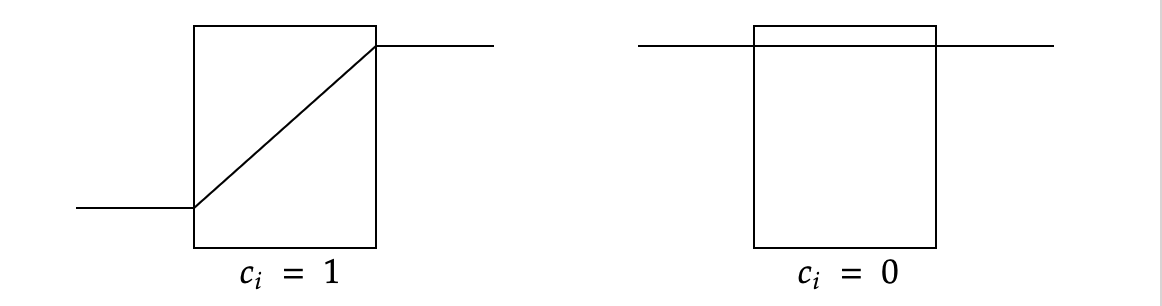
\includegraphics[scale=0.75]{cases.png}
\caption{Defines the possible values of \textit{c} for i'th Multiplexer and corresponding Multiplexer Configuration}
\end{figure}

For a Multiplexer, time delays $\displaystyle p_{i} ,\ q_{i} ,r_{i} ,\ s_{i}$ are defined as:
\begin{figure}[h]
  \centering
  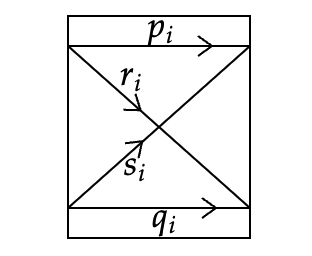
\includegraphics[scale=0.75]{delays.png}
\end{figure}
\begin{center}
  \Large $t_{i}^{u} = [ (1-c_{i})p_i + c_ir_i] + t_{i-1}^{u}$ \large(if the signal started upper at (\textit{i-1})th Multiplexer)\\
\end{center}
\begin{center}
  \Large $t_{i}^{u} = [ (1-c_{i})q_i + c_is_i] + t_{i-1}^{l}$ \large(if the signal started lower at (\textit{i-1})th Multiplexer)\\
\end{center}
\begin{center}
{where $t_{i}^{u}$ refers to the signal that comes out as upper signal at last Multiplexer}
\end{center}
Since we need the time of the signal that reaches as the upper signal we can think of it like finding out the time of the signal that starts out as upper but with the reverse challenge input given to us. So if the number of interchanges of signal from the last to the $ i^{th}$ Multiplexer is even then we need the time of the signal that enters the ith Multiplexer as the upper signal otherwise it cannot reach as upper signal and if it's odd then the lower signal at ith Multiplexer turns out to be the final upper signal\\
\\In order to know whether the final upper signal is UPPER or LOWER at the $ i^{th}$ Multiplexer, we can use the expression:
\begin{center}
  \Large$\prod_{i=i}^{31} (1-2c_i)$
\end{center}

Hence the time that the final UPPER signal takes at $ i^{th}$ Multiplexer would be:
\Large
\begin{equation}
  \begin{split}
    t_{i}^{u} &= [(1-c_{i})p_i + c_ir_i ] [\frac{1 + \prod_{i=i}^{31} (1-2c_i)}{2}] \\
              &+ [ (1-c_{i})q_i + c_is_i] [\frac{1 - \prod_{i=i}^{31} (1-2c_i)}{2}]
  \end{split}
\end{equation}
\large
which can be written as:
\Large
\begin{equation}
  \begin{split}
    t_{i}^{u} &= \frac{(1-2c_i)}{2} \frac{(p_i + q_i - r_i - s_i)}{2} + \frac{(p_i + q_i + r_i + s_i)}{4} \\
              &+ [\frac{\prod_{i=i+1}^{31} (1-2c_i)}{2}][ \frac{(p_i - q_i - r_i + s_i)}{2}] \\
              &+ [{\prod_{i=i}^{31} (1-2c_i)}][ \frac{(p_i - q_i + r_i +-s_i)}{4}]
  \end{split}
\end{equation}
\large
Using the Following Substitutions:
\Large
\begin{center}
  $\alpha_i = \frac{p_i - q_i + r_i - s_i}{4} $\\
  $\beta_i = \frac{p_i - q_i - r_i + s_i}{4} $\\
  $\gamma_i = \frac{p_i + q_i - r_i - s_i}{4}$\\
  $b_i = \frac{p_i + q_i + r_i + s_i}{4}$\\
  $d_i = (1-2c_i)$\\
  \large(i=0,1,2,...31)\\

\end{center}
\begin{center}
  \Large$w_i = \alpha_i + \beta_{i-1}$  \large(i=1,2,...31)\\
\end{center}
\begin{center}
  \Large$w_0 = \alpha_0$ \large (i=0)\\
\end{center}
\begin{center}
  \Large$x_i = d_{31}.d_{30}...d_{i+1}.d_{i} $
\end{center}
\large
Total Time (summation of time taken at each Multiplexer) would be:
\begin{center}
  \Large$T_{31}^{u} = \sum_{i=0}^{31} (d_i\gamma_i + b_i + w_ix_i) + \frac{p_{31} - q_{31} - r_{31} - s_{31}}{4}$\\
  \begin{equation}
  T_{31}^{u} = \sum_{i=0}^{31} (d_i\gamma_i + b_i + w_ix_i) + \beta_{31}
  \end{equation}
\end{center}
\large
This can be written as $W^{T}\phi(c) + b$:
\begin{center}
  \Large$w_i = \alpha_i + \beta_{i-1}$  \large(i=1,2,...30)\\
\end{center}
\begin{center}
  \Large$w_0 = \alpha_0$\\
\end{center}
\begin{center}
  \Large$w_{31} = \alpha_{31} + \beta_{31} + \gamma_{31}$\\
\end{center}
\begin{center}
  \Large$w_i = \gamma_{i-32}$  \large(for i=32, 33,... 62)\\
\end{center}
\begin{center}
  \Large$\phi_i = x_{i}$  \large(for i=0, 1,... 31)\\
\end{center}
\begin{center}
  \Large$\phi_i = d_{i-32}$  \large(for i=32, 33,... 62)\\
\end{center}
\begin{center}
  \Large$b= \sum_{i=0}^{31} b_i + \frac{p_{31} - q_{31} - r_{31} + s_{31}}{4}$\\
\end{center}
\begin{center}
  \Large$\Rightarrow W^{T}\phi(c) + b$\\
\end{center}

%%%%%%%%%%%%%%%%%%%%%%%%%%%%%%%%%%%%%%%%%%---QUESTION 2---%%%%%%%%%%%%%%%%%%%%%%%%%%%%%
\section{}
\large
\textbf{Dimensionality = 63}\\
As 63 Linearly Independent terms are included in Linear Model \textbf{W}


%%%%%%%%%%%%%%%%%%%%%%%%%%%%---QUESTION 3---%%%%%%%%%%%%%%%%%%%%%%%%%%%%%%%%
\section{}
\Large
\begin{equation}
  \begin{split}
    T_i &= t_i^{u} + t_i^{l}\\
        &= \sum_{i=0}^{i} [(p+q)(1-c_i) + (r+s)(c_i)]\\
        &= \sum_{i=0}^{i} [(p+q-r-s)(\frac{1-2c_i}{2}) + \frac{p+q+r+s}{2}]
  \end{split}
\end{equation}

\begin{equation}
  \begin{split}
    t_i^u &= \sum_{i=0}^{i}[(1-2c_i)(\frac{p_i + q_i - r_i - s_i}{4}) + \frac{p_i + q_i + r_i + s_i}{4} \\
          &+ \prod_{i=i}^{31}(1-2c_i)(\frac{p_i - q_i +r_i - s_i}{4}) + \prod_{i=i+1}^{31}(1-2c_i)(\frac{p_i - q_i -r_i + s_i}{4})]
  \end{split}
\end{equation}
\begin{equation}
  \begin{split}
    t_i^l = T_i - t_i^u &= \sum_{i=0}^{i}[(1-2c_i)(\frac{p_i + q_i - r_i - s_i}{4}) + \frac{p_i + q_i + r_i + s_i}{4} \\
                        &- \prod_{i=i}^{31} (1-2c_i)(\frac{p_i - q_i + r_i - s_i}{4}) \\
                        &- \prod_{i=i+1}^{31} (1-2c_i)(\frac{p_i - q_i - r_i + s_i}{4})]
  \end{split}
\end{equation}
\large
For PUF0, delays remain the same, $p_i, q_i, r_i, s_i$\\
For PUF1, corresponding delays are denoted as $p_i^{'}, q_i^{'}, r_i^{'}, s_i^{'}$\\
\textit{(for the $i^{'} th$ Multiplexer)}\\
Hence for Response0, if sign of $t_{31}^{l'} - t_{31}^l$ is positive, Response0 will be 1\\

Therefore, it can be written as:
\Large
\begin{center}
  $\frac{1 + sign(t_{31}^{l'} - t_{31}^l)}{2}$
\end{center}
\large
Here 
\Large
\begin{equation}
  t_{31}^{l'} - t_{31}^l = \sum_{i=0}^{31}[d_i (\gamma_i^{'} - \gamma_i) + b_i^{'} - b_i - (w_i^{'}x_i - w_ix_i)] - \beta_{31}^{'} + \beta_{31}
\end{equation}


\large This can be written as $W^{T}\phi(c) + b:$\\ ($\phi$ has the same meaning as before)

\begin{center}
  \Large$w_i = \alpha_i + \beta_{i-1} - \alpha_i^{'} - \beta_{i-1}^{'}$  \large(i=1,2,...30)\\
\end{center}
\begin{center}
  \Large$w_0 = \alpha_0 - \alpha_0^{'}$\\
\end{center}
\begin{center}
  \Large$w_{31} = \alpha_{31} + \beta_{31} + \gamma_{31} - \alpha_{31}^{'} - \beta_{31}^{'} - \gamma_{31}^{'}$\\
\end{center}
\begin{center}
  \Large$w_i = \gamma_{i-32} - \gamma_{i-32}^{'}$  \large(for i=32, 33,... 62)\\
\end{center}
\begin{center}
  \Large$\phi_i = x_{i}$  \large(for i=0, 1,... 31)\\
\end{center}
\begin{center}
  \Large$\phi_i = d_{i-32}$  \large(for i=32, 33,... 62)\\
\end{center}
\begin{center}
  \Large$b= \sum_{i=0}^{31} (b_i - b_i^{'}) + \beta_{31} - \beta_{31}^{'}$\\
\end{center}
\begin{center}
  \Large$\Rightarrow W^{T}\phi(c) + b$\\
  \large (All Other Notations are same as in Q1)
\end{center}

And For Response 1: sign of $t_{31}^u - t_{31}^{u'}$ decides the response\\
Here \Large
\begin{equation}
  t_{31}^{u} - t_{31}^{u'} = \sum_{i=0}^{31}[d_i (\gamma_i - \gamma_i^{'}) + b_i - b_i^{'} + (w_ix_i - w_i^{'}x_i)] + \beta_{31} - \beta_{31}^{'}
\end{equation}
\large This can be written as:

\begin{center}
  \Large$\Rightarrow W^{T}\phi(c) + b$\\
  \large (All Notations are same as above)
\end{center}

%%%%%%%%%%%%%%%%%%%%%%%%%%%%---QUESTION 4---%%%%%%%%%%%%%%%%%%%%%%%%%%%%%%%%
\large
\section{}
Dimensionality for Response 0 = \textbf{63}\\
Dimensionality for Response 1 = \textbf{63}\\
%%%%%%%%%%%%%%%%%%%%%%%%%%%%---QUESTION 6---%%%%%%%%%%%%%%%%%%%%%%%%%%%%%%%%
\setcounter{section}{5}
\section{}


Here we will discuss the model performance of LinearSVC and LogisticRegression considering the metrics:\\
(1) my\_fit Time : Time taken by the my\_fit() function in seconds\\
(2) 1 - Accuracy (Response 0) : Accuracy Losses for the Response 0 Arbiter PUF\\
(3) 1 - Accuracy (Response 1) : Accuracy Losses for the Response 1 Arbiter PUF

For all the above mentioned metrics, the lower the output values, the better the model performance\\
\newpage
(a) changing the loss hyperparameter in LinearSVC (hinge vs squared hinge)
\begin{figure}[H]
  \centering
  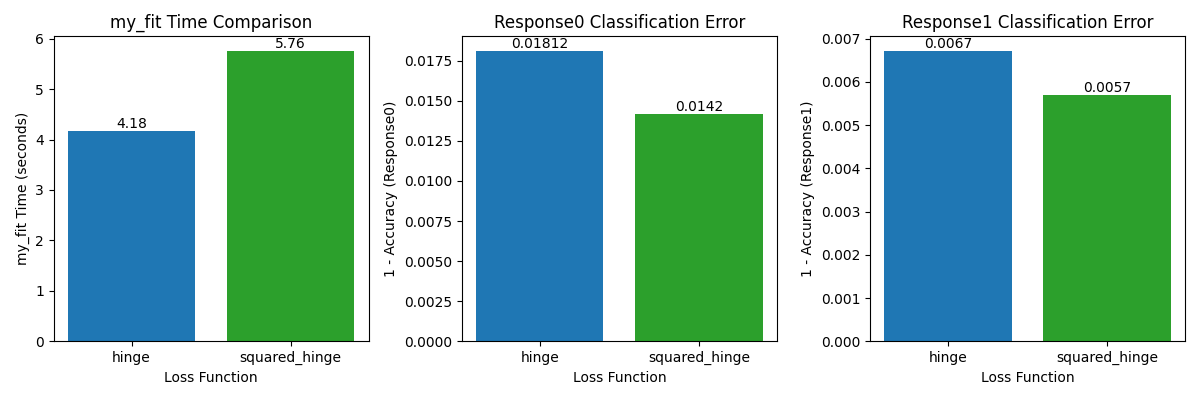
\includegraphics[scale=0.4]{loss_parameter.png}
  \caption{}
\end{figure}
(b) setting C in LinearSVC and LogisticRegression to high/low/medium values
\begin{figure}[H]
  \centering
  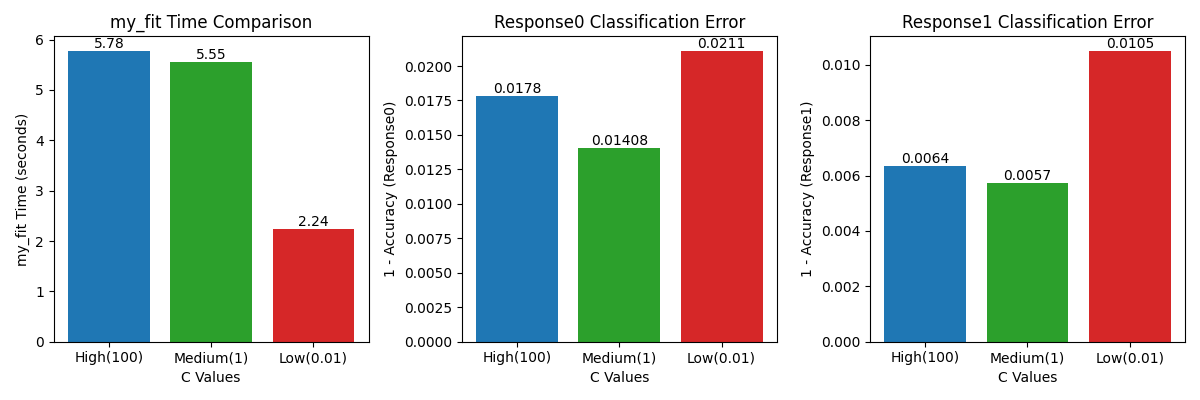
\includegraphics[scale=0.4]{C_SVC.png}
  \caption{LinearSVC model statistics with varying hyperparameter C (inverse regularization)}
  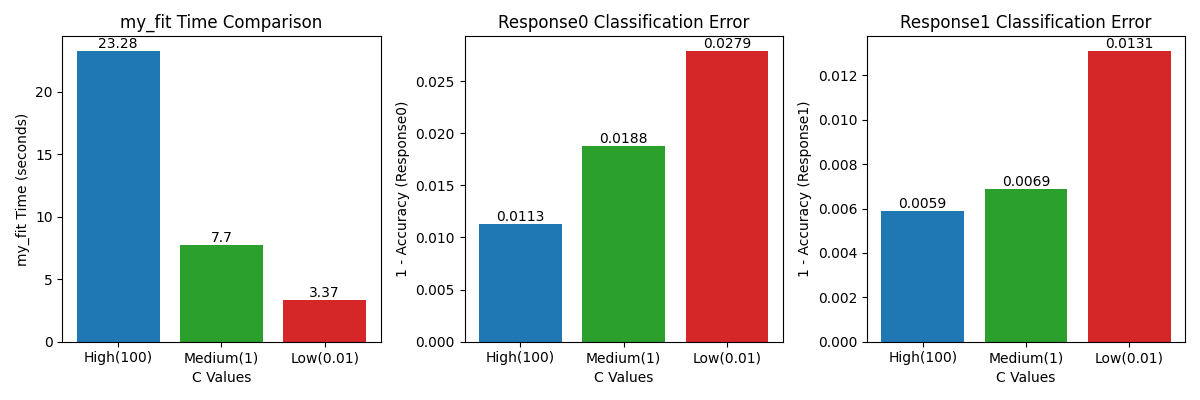
\includegraphics[scale=0.4]{C_Log.png}
  \caption{Logistic Regression model statistics with varying hyperparameter C (inverse regularization)}
\end{figure}
\newpage
(c) changing tol in LinearSVC and LogisticRegression to high/low/medium values
\begin{figure}[H]
  \centering
  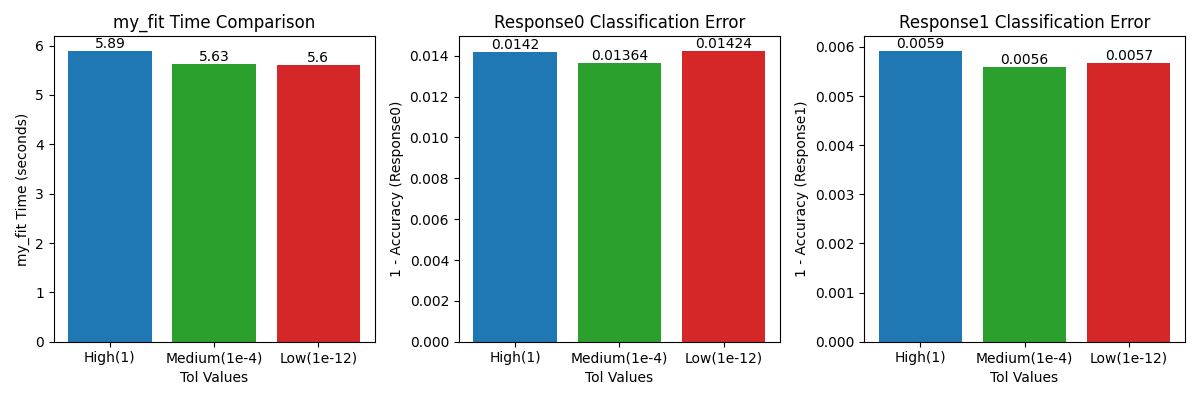
\includegraphics[scale=0.4]{tol_SVC.png}
  \caption{LinearSVC model statistics with varying Tolerance}
  \includegraphics[scale=0.4]{tol_Log.png}
  \caption{Logistic Regression model statistics with varying Tolerance}
\end{figure}

(d) changing the penalty (regularization) hyperparameter in LinearSVC and Logisti-
cRegression (l2 vs l1)

\begin{figure}[H]
  \centering
  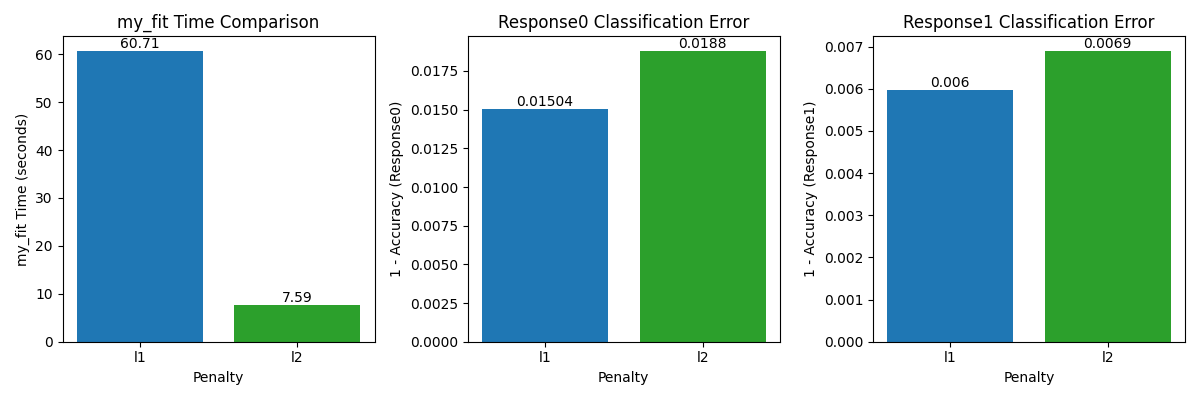
\includegraphics[scale=0.4]{penalty_svc.png}
  \caption{LinearSVC model statistics with varying norms used in penalization}
  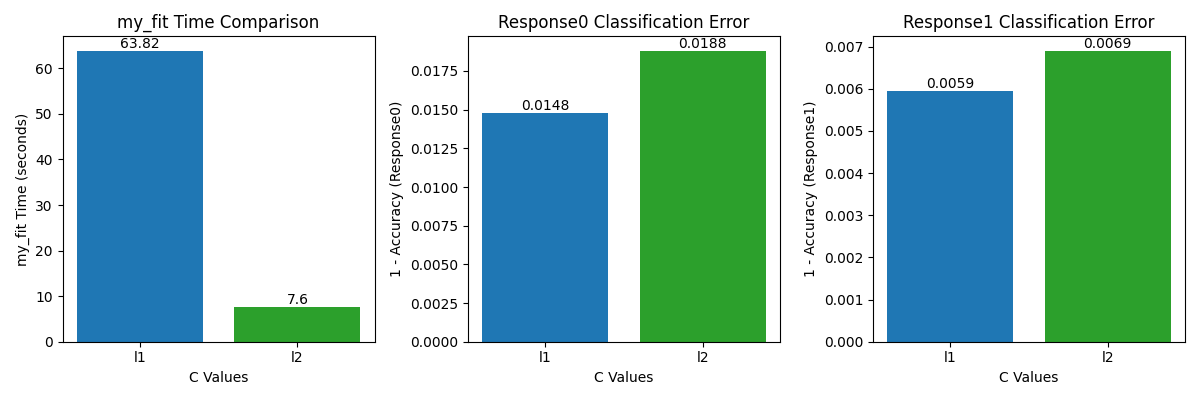
\includegraphics[scale=0.4]{penalty_log.png}
  \caption{LinearSVC model statistics with varying norms used in penalization}
\end{figure}

\section[short]{References}
  \begin{enumerate}
    \item \href{https://en.wikipedia.org/wiki/Khatri%E2%80%93Rao_product#Column-wise_Kronecker_product}{Khatri-Rao Product - Wikipedia}
    \item \href{https://matplotlib.org/stable/gallery/index.html}{matplotlib Documentation}
    \item \href{https://scikit-learn.org/stable/modules/generated/sklearn.svm.LinearSVC.html}{scikit-learn Documentation}
    \item \href{https://eprint.iacr.org/2023/287}{Modelling Delay-based Physically Unclonable Functions through Particle Swarm Optimization - \normalsize \textit{
    Nimish Mishra, Indian Institute of Technology Kharagpur,
    Kuheli Pratihar, Indian Institute of Technology Kharagpur,
    Anirban Chakraborty, Indian Institute of Technology Kharagpur,
    Debdeep Mukhopadhyay, Indian Institute of Technology Kharagpur}}
  \end{enumerate}
\end{document}